\chapter{Audio}
		In questo capitolo verrà descritto il suono, le sue caratteristiche e le sue rappresentazioni digitali, partendo dalle più comuni fino ad arrivare a quelle utilizzate per questo lavoro.
		
		\section{Il suono}
			Il suono è un segnale acustico prodotto dalle vibrazioni di un corpo e dalla trasmissione di queste attraverso un mezzo, ad esempio l’aria. Di questo segnale è possibile misurare l’intensità, ovvero la variazione di pressione, l'unità di misura più comunemente utilizzata sono i decibel (dB).
			
			Possiamo dividere i suoni in due classi: periodici e aperiodici.
			Per quanto riguarda i suoni periodici questi possono essere semplici, come delle onde sinusoidali, o complessi, risultato di più onde sinusoidali combinate.
			Mentre i suoni aperiodici non presentano pattern ripetitivi e possono essere continui, come il rumore, o transienti, come impulsi.
			
		\section{Onda sinusoidale}
			Al fine di poter descrivere al meglio cos'è il suono, è necessario definirlo nella sua forma più semplice: l'onda sinusoidale. Essa consiste in un suono periodico semplice, descrivibile con la seguente formula:
			\begin{equation}
				y(t) = A \cdot sin(2 \pi ft + \varphi)
			\end{equation}
			I parametri fondamentali al fine di caratterizzare un'onda sinusoidale dunque sono:
			\begin{enumerate}
				\item \textbf{Frequenza} (f): La frequenza di un suono è un concetto che si basa sulla periodicità di un segnale ed è espresso come l'inverso del tempo che esso impiega a ripetersi, ovvero a compiere un ciclo ($f=1/T$).
				\item \textbf{Ampiezza} (A): L'ampiezza di un segnale è la misurazione della variazione di pressione dello stesso.
				\item \textbf{Fase} ($\varphi$): La fase di un segnale rappresenta la quantità di frazione di un ciclo, quindi una completa oscillazione, compiuta dall'onda.
			\end{enumerate}
			
		\section{Digitalizzazione segnale audio}
			Al fine di poter rappresentare digitalmente questi segnali analogici, abbiamo bisogno di un campionamento (Fig. \ref{fig:campionamento}).
			Esso consiste nel misurare e registrare la pressione sonora del segnale acustico ogni T secondi, tale valore viene definito come \textit{intervallo di campionamento}. Il numero di campioni che registriamo in un secondo viene definita \textit{frequenza di campionamento}.
			
			Il teorema di Nyquist-Shannon definisce la frequenza massima rappresentabile $f_{N}$ (frequenza di Nyquist) dato un campionamento con una frequenza $f_{s}$ senza perdita di informazione.
			\begin{equation}
				f_{N} = \frac{1}{2} f_{s}
				\label{eq:fn}
			\end{equation}
			
			Nonostante questa tipologia di codifica dell'audio risulti ottimale per la conversione analogico-digitale dei segnali, non ci permette agilmente di ottenere quelle che sono le feature più interessanti per la nostra percezione.
			\begin{figure}%[h]
	\centering
	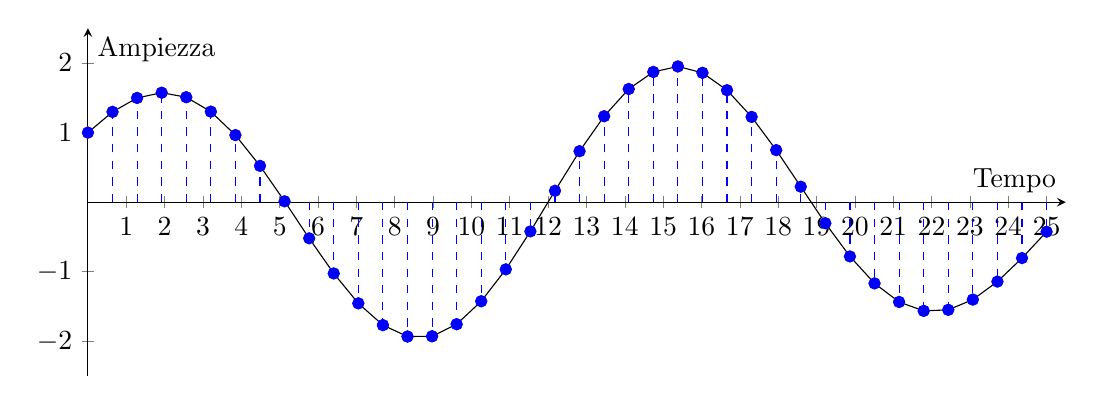
\begin{tikzpicture}[>=latex]
		\begin{axis}[
			axis lines = middle,
			xlabel = Tempo,
			ylabel = Ampiezza,
			xtick={0,1,...,25},
			ytick={-2,-1,...,2},
			xmin=0,
			xmax=25.5,
			ymin=-2.5,
			ymax=2.5,
			width=140mm,
			height=60mm,
			]
			\addplot[
			scatter,
			domain=0:25,
			samples=40,
			color=black
			]
			{sin(180*x/6)+cos(180*x/8)};
			\addplot[
			only marks,
			domain=0:25,
			samples=40,
			color=blue
			]{sin(180*x/6)+cos(180*x/8)};
			\addplot[
			ycomb,
			dashed,
			domain=0:25,
			samples=40,
			color=blue
			]
			{sin(180*x/6)+cos(180*x/8)};
		\end{axis}
	\end{tikzpicture}
	\caption{Campionamento di un segnale audio complesso. L'onda viene scomposta in campioni equidistanti che rappresentino l'ampiezza nel tempo, descrivendo l'onda originale.}
	\label{fig:campionamento}
\end{figure}
			
		\section{Spettrogramma}
		Uno spettrogramma è una rappresentazione dello spettro di potenza di un segnale audio sul dominio del tempo (Fig. \ref{fig:spettrogramma}). Al fine di definire uno spettrogramma, è dunque necessario prima descrivere cosa sia uno spettro di potenza. Esso consiste nella rappresentazione di un segnale audio in un certo istante temporale $t$ in funzione della frequenza.
				
		Il metodo più veloce per calcolare lo spettro di potenza di un segnale audio è attraverso la \textit{fast Fourier transform} (FFT), un algoritmo che calcola la \textit{trasformata discreta di Fourier} (DFT) con costo computazionale $O(n \cdot log(n))$\cite{audio-fft}.
		\begin{figure}[h]
			\centering
			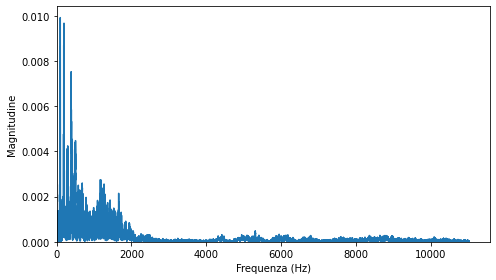
\includegraphics[width=0.75\linewidth]{figures/spectrum}
			\caption{Spettro di potenza di una voce maschile pronunciando "It's not forever".}
			\label{fig:spettro}
		\end{figure}
		Calcolando la DFT sull'intero audio otteniamo dunque lo spettro dell'intero segnale audio analizzato (Fig. \ref{fig:spettro}) ma non possiamo sapere in quale istante sono avvenuti i principali picchi.
		
		Per ovviare a questo problema di mancanza di riferimento temporale, dobbiamo calcolare la DFT su porzioni di audio in sequenza temporale. Questa operazione viene definita \textit{short-time fourier transform} (STFT) e possiamo così visualizzarne il risultato sotto forma di spettrogrammi (Fig. \ref{fig:spettrogramma})\cite{time-frequency-review}.
		
		 Uno spettrogramma può essere rappresentato con una heat map in cui gli assi descrivono la frequenza e il tempo, mentre l'intensità sonora è espressa attraverso il colore. Questo tipo di codifica ci permette quindi di accedere ad informazioni più rilevanti riguardo il suono in uno spazio ristretto.
		\begin{figure}%[h]
			\centering
			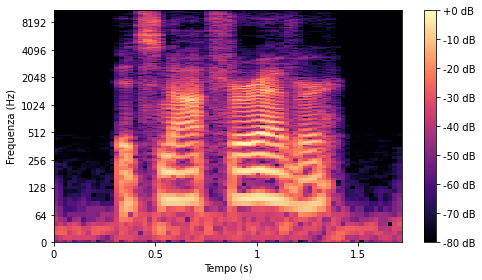
\includegraphics[width=0.75\linewidth]{figures/spectrogram}
			\caption{Spettrogramma di una voce maschile pronunciando "It's not forever".}
			\label{fig:spettrogramma}
		\end{figure}
	
		\section{Spettrogramma mel}
		 Tuttavia è importante considerare come la percezione umana del suono non sia lineare ma sia dipendente dall'altezza sonora (pitch) e quindi dalla frequenza dei suoni che udiamo. La scala mel viene per la prima volta sviluppata nel 1937 in una ricerca effettuata da Stevens e consiste in una scala di frequenze con altezze diverse (pitch) giudicate dagli ascoltatori come equidistanti (Fig. \ref{fig:scala-mel})\cite{Stevens1937}.
		 Non esiste propriamente una formula per la scala di mel ma tra le più comuni troviamo:
		 \begin{equation}
		 	mel(x) = 2595 \log_{10}(1+\frac{x}{700})
		 \end{equation}
		 \newcommand{\vertLineFromPoint}[1]{
	\draw[dashed] 
	(#1) -- (#1|-{rel axis cs:0,0})
}
\newcommand{\horLineFromPoint}[1]{
	\draw[dashed] 
	(#1) -- (#1-|{rel axis cs:0,0})
}
\begin{figure}[h]
	\centering
	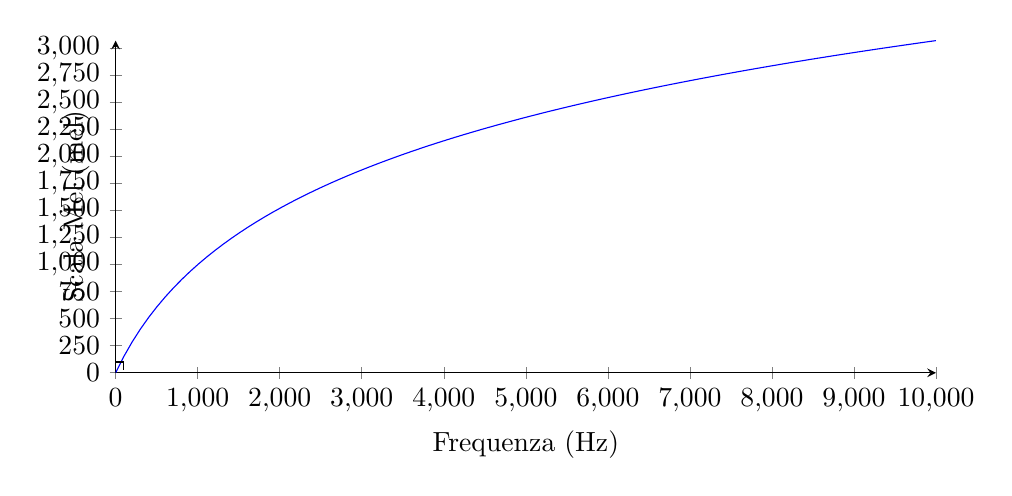
\begin{tikzpicture}
		\begin{axis}[
			width=120mm,
			height=58mm,
			axis lines=left,
			domain=0:10000,
			samples=100,
			no markers,
			xlabel=Frequenza (Hz),
			ylabel=Scala Mel (mel),
			y label style={at={(axis description cs:-0.02,.5)}},
			xtick distance=1000,
			ytick distance=250
			]
			\addplot {2595 * log10(1+x/700)};
			\vertLineFromPoint{100,100};
			\horLineFromPoint{100,100};
		\end{axis}
	\end{tikzpicture}
	\caption{Grafico della scala mel.}
	\label{fig:scala-mel}
\end{figure}
	 	
		Possiamo quindi impiegare questa scala per realizzare una rappresentazione che ci consentirà in fase di elaborazione di ottenere manipolazioni più significative per il nostro apparato uditivo (Fig. \ref{fig:spettrogramma-mel}).
		
		L'inversione degli spettrogrammi è soggetta alla produzione di artefatti in quanto nel calcolo della trasformata discreta di Fourier si ha perdita di informazione delle fasi dei segnali. Tuttavia grazie allo sviluppo recente di vocoder neurali, come MelGAN\cite{melgan}, in grado di rigenerare correttamente l'audio a partire da spettrogrammi mel, questi sono diventati sempre più di uso comune.
		\begin{figure}%[h]
			\centering
			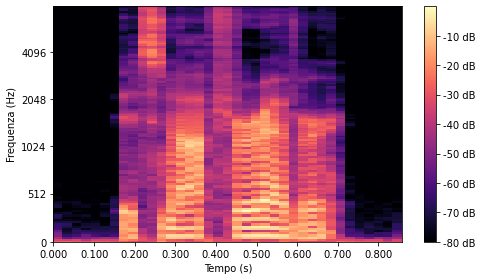
\includegraphics[width=0.75\linewidth]{figures/melspectrogram}
			\caption{Spettrogramma mel di una voce maschile pronunciando "It's not forever".}
			\label{fig:spettrogramma-mel}
		\end{figure}
	
		\section{Coefficienti mel-frequency cepstrum}
		I coefficienti mel-frequency cepstrum (MFCC)\cite{mel-frequency-cepstral} sono una rappresentazione dell'audio largamente usato nello speech processing tradizionale che ha trovato largo utilizzo anche nel machine learning, come nella speech recognition. Al fine di ottenere un MFCC è sufficiente calcolare la \textit{trasformata discreta del coseno} (DCT) dello spettrogramma mel dell'audio desiderato (Fig. \ref{fig:mfcc}).
		\begin{figure}%[h]
			\centering
			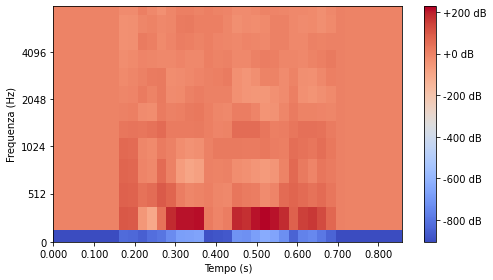
\includegraphics[width=0.75\linewidth]{figures/mfcc}
			\caption{MFCC di una voce maschile pronunciando "It's not forever".}
			\label{fig:mfcc}
		\end{figure}
		
		\section{Sine-wave speech}
		La sine-wave speech (SWS) è una forma di audio del parlato umano a spettro ridotto, in cui vi sono presenti in genere tre o quattro componenti sinusoidali mobili (Fig. \ref{fig:sine-wave-speech}). L'audio viene generato rimpiazzando le formanti con delle sinusoidi al fine di rimuovere il più possibile la componente acustica mantenendo però intelligibilità.
		\begin{figure}[h]
			\centering
			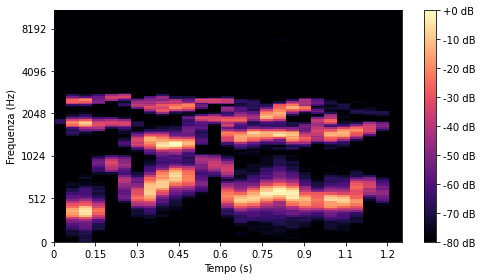
\includegraphics[width=0.75\linewidth]{figures/sine-wave_speech}
			\caption{Spettrogramma mel di una voce maschile pronunciando "It's not forever" in SWS con 3 componenti.}
			\label{fig:sine-wave-speech}
		\end{figure}
	
		Viene per la prima volta sviluppato negli Haskins Laboratories da Rubin\cite{haskins-laboratories} e successivamente impiegato in vari esperimenti riguardanti la percezione del parlato, come da Remez et al. che nel 1981 dimostrò come nonostante la sua apparente forma innaturale, la sine-wave speech conservi le proprietà sufficienti per la percezione del contenuto linguistico\cite{remez1981speech}.
		
		\section{Vocoded speech}
		Il vocoder è una tecnica di elaborazione dell'audio che richiede due sorgenti: un carrier, che accoglierà il suono, e un modulatore, che darà forma al suono del carrier. Le caratteristiche armoniche del modulatore vengono codificate all'interno del carrier, ottenendo un segnale con uno spettro alterato (Fig. \ref{fig:buzz-vocoded} e \ref{fig:noise-vocoded}).
		
		Le ricerche sulla percezione del parlato in condizioni di alterazione spettrale trovano il loro interesse anche per questa forma di modulazione. Il lavoro di Davis et al. sulla comprensione del parlato noise-vocoded dimostra come anche in questo caso, l'ascoltatore impari a riconoscere il parlato nonostante la forte distorsione di esso\cite{noise-vocoded}.
		\begin{figure}%[h]
			\centering
			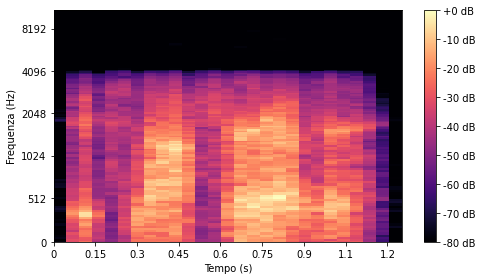
\includegraphics[width=0.75\linewidth]{figures/noise-vocoded}
			\caption{Vocoder con noise come carrier e una voce maschile pronunciando "It's not forever" come modulatore.}
			\label{fig:noise-vocoded}
		\end{figure}
		\begin{figure}%[h]
			\centering
			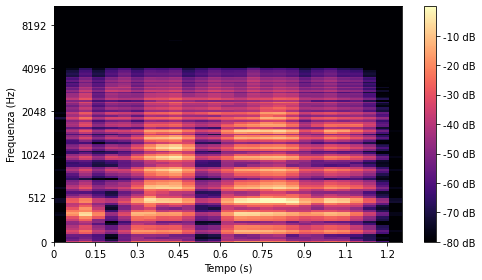
\includegraphics[width=0.75\linewidth]{figures/buzz-vocoded}
			\caption{Vocoder con un buzz a 500 Hz come carrier e una voce maschile pronunciando "It's not forever" come modulatore.}
			\label{fig:buzz-vocoded}
		\end{figure}
	